\documentclass{article}
\usepackage[utf8]{inputenc}
\usepackage[shortlabels]{enumitem}
\usepackage{geometry}
\geometry{a4paper,left=20mm,right=20mm, top=10mm}
\usepackage{graphicx}
\usepackage{float}
\usepackage{amsmath}
\usepackage{bm}
\usepackage{dsfont}
\usepackage{upgreek}
\usepackage{float}
\usepackage{xcolor}
%\usepackage{color}
\usepackage{subcaption}
\usepackage{graphicx} 
\usepackage{hyperref}
\usepackage{tikz}
\usetikzlibrary{arrows}
\usepackage{array}
\setlength\parindent{0pt}
\usepackage{multirow}
\usepackage{makecell}

\renewcommand\cellalign{cl}
\begin{document}


\begin{figure}[H]
    \centering
    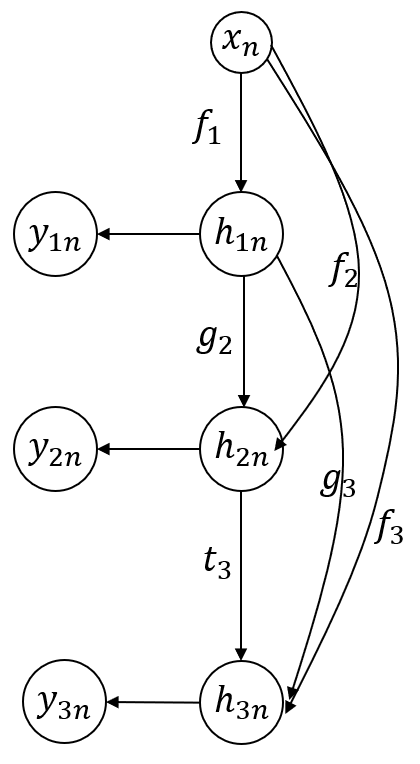
\includegraphics[width=0.3\textwidth]{new.PNG}
    \caption{GPLAR with separate GPs}
\end{figure}

As shown in Figure 1, $h_{2n}$ is generated by sum of two Gaussian process value, which is the following:

\begin{align*}
    p(h_{1n}) &= \mathcal{N}(h_{1n};f_1(\mathbf{x}_n), \sigma^2)\\
    p(h_{2n}) &= \mathcal{N}(h_{2n};f_2(\mathbf{x}_n)+g_2(h_{1n}), \sigma^2)\\
    p(h_{3n}) &= \mathcal{N}(h_{3n};f_3(\mathbf{x}_n)+g_3(h_{1n})+t_3(h_{2n}), \sigma^2)
\end{align*}

Introducing inducing-points into each GP function, we have the approximate posterior and the complete probability of the model as follows,

\begin{align*}
    p(f_{1:3},g_{2:3}, t_3, \mathbf{h}_{1:3}, \mathbf{y}_{1:3}) =&
    p(f_{1\neq \mathbf{u}_1}|\mathbf{u}_1)p(\mathbf{u}_1)\\
    & p(f_{2\neq \mathbf{u}_2}|\mathbf{u}_2)p(\mathbf{u}_2) p(g_{2\neq \mathbf{v}_2}|\mathbf{v}_2)p(\mathbf{v}_2)\\
    & p(f_{3\neq \mathbf{u}_3}|\mathbf{u}_3)p(\mathbf{u}_3) p(g_{3\neq \mathbf{v}_3}|\mathbf{v}_3)p(\mathbf{v}_3) p(t_{3\neq \mathbf{w}_3}|\mathbf{w}_3)p(\mathbf{w}_3)\times\\
    & \prod_n p(h_{1n}|f_1,\mathbf{x}_n) p(h_{2n}|f_2, g_2, \mathbf{x}_n, h_{1n}) p(h_{3n}|f_3,g_3,t_3, \mathbf{x}_n, h_{1n}, h_{2n})\\
    & \hspace{1.5em} p(y_{1n}|h_{1n})p(y_{2n}|h_{2n})p(y_{3n}|h_{3n})\\
    \\
    q(f_{1:3},g_{2:3}, t_3, \mathbf{h}_{1:3}) =&
    p(f_{1\neq \mathbf{u}_1}|\mathbf{u}_1)q(\mathbf{u}_1)\\
    & p(f_{2\neq \mathbf{u}_2}|\mathbf{u}_2)q(\mathbf{u}_2) p(g_{2\neq \mathbf{v}_2}|\mathbf{v}_2)q(\mathbf{v}_2)\\
    & p(f_{3\neq \mathbf{u}_3}|\mathbf{u}_3)q(\mathbf{u}_3) p(g_{3\neq \mathbf{v}_3}|\mathbf{v}_3)q(\mathbf{v}_3) p(t_{3\neq \mathbf{w}_3}|\mathbf{w}_3)q(\mathbf{w}_3)\times\\
    & \prod_n p(h_{1n}|f_1,\mathbf{x}_n) p(h_{2n}|f_2, g_2, \mathbf{x}_n, h_{1n}) p(h_{3n}|f_3,g_3,t_3, \mathbf{x}_n, h_{1n}, h_{2n})
\end{align*}

Lower bound to the marginal log-likelihood becomes,

\begin{align*}
    \mathcal{L}_{ELBO} &=  \mathds{E}_q\left[\log\frac{p(f_{1:3},g_{2:3}, t_3, \mathbf{h}_{1:3}, \mathbf{y}_{1:3})}{q(f_{1:3},g_{2:3}, t_3, \mathbf{h}_{1:3})}\right]\\
    &= \sum_{l,n} \mathds{E}_q \log p(y_{ln}|h_{ln}) - \sum_{l=1}^3 KL\left[q(\mathbf{u}_l)\|p(\mathbf{u}_l)\right] - \sum_{l=2}^3 KL\left[q(\mathbf{v}_l)\|p(\mathbf{v}_l)\right] - \sum_{l=3}^3 KL\left[q(\mathbf{w}_l)\|p(\mathbf{w}_l)\right]
\end{align*}

where the expectation log-term requires computation of the following:

\begin{align*}
    \int & p(f^{1}_{l\neq\mathbf{u}_l^1}|\mathbf{u}_l^1)q(u_l^1)\dots
    p(f^{l}_{l\neq\mathbf{u}_l^l}|\mathbf{u}_l^l)q(u_l^l) p(h_{ln}|f_l^{1...l},\mathbf{x}_n,h_{1n,...,(l-1)n})\\
    & q(h_{1n}) q(h_{2n}|h_{1n})\dots q(h_{(l-1)n}|h_{1n}\dots h_{(l-2)n})\\ 
    & \log p(y_{ln}|h_{ln}) d\mathbf{h}
\end{align*}

where $p(h_{ln}|f_l^{1...l},\mathbf{x}_n,h_{1n,...,(l-1)n}) = \mathcal{N}(h_{ln}; f_l^1(\mathbf{x}_n) + f_l^2(h_{1n}) + \dots + f_l^l(h_{(l-1)n}), \sigma^2)$ and the function $f_l^{1...l}$ can be integrated out analytically as follows,

\begin{align*}
    q(h_{ln}|h_{1n},\dots,h_{(l-1)n}) &= \int  p(f^{1}_{l\neq\mathbf{u}_l^1}|\mathbf{u}_l^1)q(u_l^1)\dots
    p(f^{l}_{l\neq\mathbf{u}_l^l}|\mathbf{u}_l^l)q(u_l^l) p(h_{ln}|f_l^{1...l},\mathbf{x}_n,h_{1n,...,(l-1)n}) df\\
    &= \mathcal{N}(h_{ln}; \mu_l(\hat{\mathbf{x}}_n), \sigma^2_l(\hat{\mathbf{x}}_n))
\end{align*}

where,
\begin{align*}
    \mu_l(\hat{\mathbf{x}}_n) = & K_l^1(\mathbf{x}_n,\mathbf{Z}_l^1)K_l^1(\mathbf{Z}_l^1,\mathbf{Z}_l^1)^{-1}\mathbf{m}_l^1 + K_l^2(h_{1n},\mathbf{Z}_l^2)K_l^2(\mathbf{Z}_l^2,\mathbf{Z}_l^2)^{-1}\mathbf{m}_l^2 + \dots + K_l^l(h_{(l-1)n},\mathbf{Z}_l^l)K_l^l(\mathbf{Z}_l^l,\mathbf{Z}_l^l)^{-1}\mathbf{m}_l^l\\
    \sigma^2_l(\hat{\mathbf{x}}_n) = & K_l^1(\mathbf{x}_n,\mathbf{x}_n)+ K_l^1(\mathbf{x}_n,\mathbf{Z}_l^1)K_l^1(\mathbf{Z}_l^1,\mathbf{Z}_l^1)^{-1}(K_l^1(\mathbf{Z}_l^1,\mathbf{Z}_l^1)-\mathbf{S}_l^1)K_l^1(\mathbf{Z}_l^1,\mathbf{Z}_l^1)^{-1}K_l^1(\mathbf{Z}_l^1,\mathbf{x}_n)\\
    &+ K_l^2(h_{1n},h_{1n})+ K_l^2(h_{1n},\mathbf{Z}_l^2)K_l^2(\mathbf{Z}_l^2,\mathbf{Z}_l^2)^{-1}(K_l^2(\mathbf{Z}_l^2,\mathbf{Z}_l^2)-\mathbf{S}_l^2)K_l^2(\mathbf{Z}_l^2,\mathbf{Z}_l^2)^{-1}K_l^2(\mathbf{Z}_l^2,h_{1n})\\
    & + \dots \\
    &+ K_l^l(h_{(l-1)n},h_{(l-1)n})+ K_l^l(h_{(l-1)n},\mathbf{Z}_l^l)K_l^l(\mathbf{Z}_l^l,\mathbf{Z}_l^l)^{-1}(K_l^l(\mathbf{Z}_l^l,\mathbf{Z}_l^l)-\mathbf{S}_l^l)K_l^l(\mathbf{Z}_l^l,\mathbf{Z}_l^l)^{-1}K_l^l(\mathbf{Z}_l^l,h_{(l-1)n})\\
    &+ \sigma^2
\end{align*}

Here, $\mathbf{Z}_l^2 \dots \mathbf{Z}_l^l$ will be vectors, since input is univariate.\\

Model 1: Forward direction is in red, backward direction is in black, observations are in bold:

\begin{table}[H]
\centering
\begin{tabular}{|c|c|c|c|c|}
	\hline
	$\mathbf{h_{1n}}:$ & $g_1(x_n)$ & $\color{red} h_{13}(g_3(x_n))$ & $\color{red} h_{12}(g_2(x_n))$ & $\color{red} h_{123}(h_{23}(g_3(x_n)))$\\
	\hline
	$\mathbf{h_{2n}}:$ & $g_2(x_n)$ & $h_{21}(g_1(x_n))$ & $\color{red} h_{23}(g_3(x_n))$\\
	\hline
	$\mathbf{h_{3n}}:$ & $g_3(x_n)$ & $h_{31}(g_1(x_n))$ & $h_{32}(g_2(x_n))$ & $ h_{321}(h_{21}(g_1(x_n)))$\\
	\hline
	
\end{tabular}
\end{table}

The number of GPs will explode as the Pascal's Triangle.\\

The above model can also be relaxed as Model 2:
\begin{table}[H]
\centering
\begin{tabular}{|c|c|c|c|c|c|c|}
	\hline
	$t_{1n}:$ & & & $\color{blue} g_1(x_n)$ & $\color{red} g_{13}(b_{3n})$ & $\color{red} g_{12}(b_{2n})$  & $:b_{1n}$\\
	\hline
	$t_{2n}:$ & & $g_{21}(t_{1n})$ & $\color{blue} g_2(x_n)$ & $\color{red} g_{23}(b_{3n})$ &  & $:b_{2n}$\\
	\hline
	$t_{3n}:$ &$g_{32}(t_{2n})$ & $g_{31}(t_{1n})$ & $\color{blue} g_3(x_n)$ &  &  & $:b_{1n}$\\
	\hline
\end{tabular}
\end{table}

where the hidden variables in two directions share the GP over input as follows,

\begin{align*}
	t_{1n} &= g_1(x_n)\\
	t_{2n} &= g_2(x_n) + g_{21}(t_{1n})\\
	t_{3n} &= g_3(x_n) + g_{32}(t_{2n}) + g_{31}(t_{1n})\\
	\\
	b_{3n} &= g_3(x_n)\\
	b_{2n} &= g_2(x_n) + g_{23}(b_{3n})\\
	b_{3n} &= g_1(x_n) + g_{12}(b_{2n}) + g_{13}(b_{3n})\\
	\\
	h_{1n} &= g_1(x_n) + g_{12}(b_{2n}) + g_{13}(b_{3n})\\
	h_{2n} &= g_2(x_n) + g_{21}(t_{1n}) + g_{23}(b_{3n})\\
	h_{3n} &= g_3(x_n) + g_{32}(t_{2n}) + g_{31}(t_{1n})
\end{align*}

Just like Model 1, Model 2's backwards direction does not have any duplicated function over time. The number of GPs is $L^2$, where $L$ is number of outputs. However, the dependencies will still run through aggregated hidden variables, except that time and each previous output are explicitly separated.\\

For Model 1 forward version:

\begin{figure}[H]
\centering
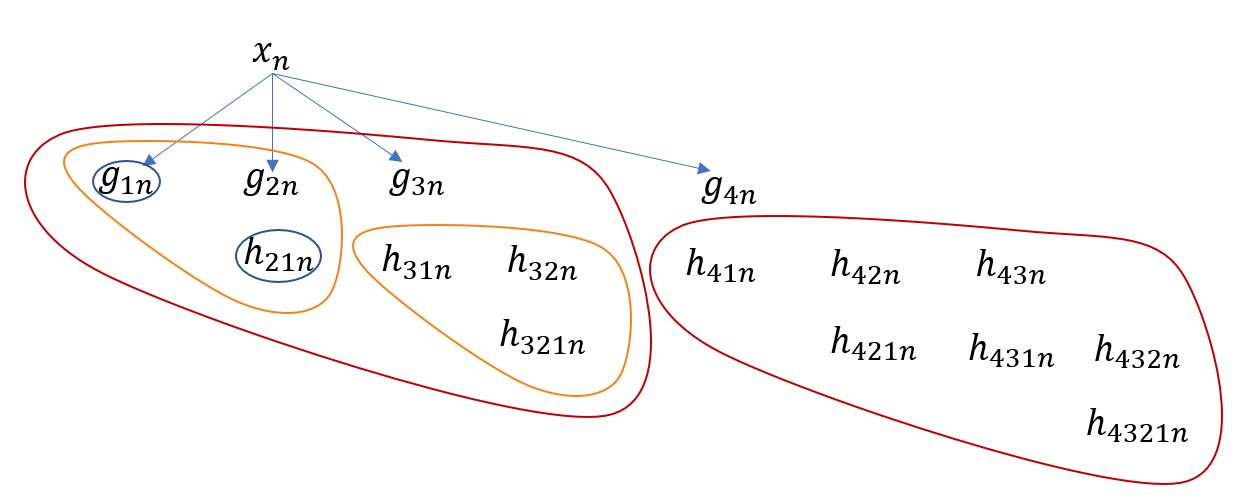
\includegraphics[width=0.7\textwidth]{new2.png}
\end{figure}

\begin{align*}
	p(\mathbf{y},g_{1:3}, h_{21,31,32,321}) = &  p(g_{1\neq\mathbf{u}_1}|\mathbf{u}_1)p(g_{2\neq\mathbf{u}_2}|\mathbf{u}_2)p(g_{3\neq\mathbf{u}_3}|\mathbf{u}_3)p(\mathbf{u}_1)p(\mathbf{u}_2)p(\mathbf{u}_3)\\	
	& p(h_{21\neq\mathbf{v}_1}|\mathbf{v}_1)p(h_{31\neq\mathbf{v}_2}|\mathbf{v}_2)p(h_{32\neq\mathbf{v}_3}|\mathbf{v}_3)p(\mathbf{v}_1)p(\mathbf{v}_2)p(\mathbf{v}_3)\\	
    & p(h_{321\neq\mathbf{w}_1}|\mathbf{w}_1)p(\mathbf{w}_1)\\
    & \prod_n p(y_{1n};g_1(x_n), \sigma^2_1)\\
    & \hspace{1.5em} p(y_{2n};g_2(x_n) + h_{21}(g_1(x_n)), \sigma^2_2)\\
    & \hspace{1.5em} p(y_{3n};g_3(x_n) + h_{31}(g_1(x_n)) + h_{32}(g_2(x_n)) + h_{321}(h_{21}(g_1(x_n))), \sigma^2_3)
\end{align*}

\begin{align*}
	q(g_{1:3}, h_{21, 31, 321}) = & p(g_{1\neq\mathbf{u}_1}|\mathbf{u}_1)p(g_{2\neq\mathbf{u}_2}|\mathbf{u}_2)p(g_{3\neq\mathbf{u}_3}|\mathbf{u}_3)q(\mathbf{u}_1)q(\mathbf{u}_2)q(\mathbf{u}_3)\\
	& p(h_{21\neq\mathbf{v}_1}|\mathbf{v}_1)p(h_{31\neq\mathbf{v}_2}|\mathbf{v}_2)p(h_{32\neq\mathbf{v}_3}|\mathbf{v}_3)q(\mathbf{v}_1)q(\mathbf{v}_2)q(\mathbf{v}_3)\\	
	& p(h_{321\neq\mathbf{w}_1}|\mathbf{w}_1)q(\mathbf{w}_1)\\
\end{align*}

\begin{align*}
	\mathcal{L}_{ELBO} = & \mathds{E}_q\left[ \frac{p(\mathbf{y},g_{1:3}, h_{21,31,32,321})}{q(g_{1:3}, h_{21, 31, 321})}\right]\\
	=  & \sum_n \int q(g_{1n}|x_n) \log p(y_{1n}|g_{1n}, \sigma^2_1) \\
	& + \sum_n \int q(g_{1n}|x_n) q(g_{2n}|x_n) q(h_{21n}|g_{1n}) \log p(y_{2n}|g_{2n},h_{21n},\sigma^2_2) \\
	& + \sum_n \int q(g_{1n}|x_n)  q(g_{2n}|x_n) q(g_{3n}|x_n)\\
	& \hspace{4em} q(h_{21n}|g_{1n}) q(h_{31n}|g_{1n}) q(h_{32n}|g_{2n}) q(h_{321n}|h_{21n}) \log p(y_{3n}| g_{3n}, h_{31n}, h_{32n}, h_{321n}, \sigma^2_3)\\
	& -\sum_{\mathbf{u}: \text{\footnotesize all inducing points}} KL(q(\mathbf{u})\|p(\mathbf{u}))
\end{align*}

where $q(\cdot|\cdot)$ is the variational posterior with inducing points analytically marginalized out. The following table shows the space where each GP's inducing inputs should lie.

\begin{table}[H]
\centering
\begin{tabular}{|c|c|c|c|}
\hline
$g_{1:3}$ & $\mathcal{X}$\\
$h_{21,31}$ & $g_1(\mathcal{X})$\\
$h_{32}$ & $g_2(\mathcal{X})$\\
$h_{321}$ & $h_{21}(g_2(\mathcal{X}))$\\
\hline
\end{tabular}
\end{table}

If bi-directional is implemented, the expectation log-term will be:

\begin{align*}
	& \sum_n \int q(g_{1n}|x_n)q(g_{2n}|x_n)q(g_{3n}|x_n)\\
	& \hspace{4em} \bigg[ \int  q(h_{13n}|g_{3n}) q(h_{12n}|g_{2n}) q(h_{23n}|g_{3n}) q(h_{123n}|h_{23n}) \log p(y_{1n}|g_{1n}, h_{13n}, h_{12n}, h_{123n}, \sigma_1^2)\\
	& \hspace{4em} \int q(h_{21n}|g_{1n}) q(h_{23n}|g_{3n}) \log p(y_{2n}|g_{2n}, h_{21n}, h_{23n}, \sigma^2_2)\\
	& \hspace{4em} \int q(h_{21n}|g_{1n}) q(h_{31n}|g_{1n}) q(h_{32n}|g_{2n}) q(h_{321n}|h_{21n}) \log p(y_{3n}| g_{3n}, h_{31n}, h_{32n}, h_{321n}, \sigma^2_3) \bigg]
\end{align*}

\end{document}


